\documentclass[1p]{elsarticle_modified}
%\bibliographystyle{elsarticle-num}

%\usepackage[colorlinks]{hyperref}
%\usepackage{abbrmath_seonhwa} %\Abb, \Ascr, \Acal ,\Abf, \Afrak
\usepackage{amsfonts}
\usepackage{amssymb}
\usepackage{amsmath}
\usepackage{amsthm}
\usepackage{scalefnt}
\usepackage{amsbsy}
\usepackage{kotex}
\usepackage{caption}
\usepackage{subfig}
\usepackage{color}
\usepackage{graphicx}
\usepackage{xcolor} %% white, black, red, green, blue, cyan, magenta, yellow
\usepackage{float}
\usepackage{setspace}
\usepackage{hyperref}

\usepackage{tikz}
\usetikzlibrary{arrows}

\usepackage{multirow}
\usepackage{array} % fixed length table
\usepackage{hhline}

%%%%%%%%%%%%%%%%%%%%%
\makeatletter
\renewcommand*\env@matrix[1][\arraystretch]{%
	\edef\arraystretch{#1}%
	\hskip -\arraycolsep
	\let\@ifnextchar\new@ifnextchar
	\array{*\c@MaxMatrixCols c}}
\makeatother %https://tex.stackexchange.com/questions/14071/how-can-i-increase-the-line-spacing-in-a-matrix
%%%%%%%%%%%%%%%

\usepackage[normalem]{ulem}

\newcommand{\msout}[1]{\ifmmode\text{\sout{\ensuremath{#1}}}\else\sout{#1}\fi}
%SOURCE: \msout is \stkout macro in https://tex.stackexchange.com/questions/20609/strikeout-in-math-mode

\newcommand{\cancel}[1]{
	\ifmmode
	{\color{red}\msout{#1}}
	\else
	{\color{red}\sout{#1}}
	\fi
}

\newcommand{\add}[1]{
	{\color{blue}\uwave{#1}}
}

\newcommand{\replace}[2]{
	\ifmmode
	{\color{red}\msout{#1}}{\color{blue}\uwave{#2}}
	\else
	{\color{red}\sout{#1}}{\color{blue}\uwave{#2}}
	\fi
}

\newcommand{\Sol}{\mathcal{S}} %segment
\newcommand{\D}{D} %diagram
\newcommand{\A}{\mathcal{A}} %arc


%%%%%%%%%%%%%%%%%%%%%%%%%%%%%5 test

\def\sl{\operatorname{\textup{SL}}(2,\Cbb)}
\def\psl{\operatorname{\textup{PSL}}(2,\Cbb)}
\def\quan{\mkern 1mu \triangleright \mkern 1mu}

\theoremstyle{definition}
\newtheorem{thm}{Theorem}[section]
\newtheorem{prop}[thm]{Proposition}
\newtheorem{lem}[thm]{Lemma}
\newtheorem{ques}[thm]{Question}
\newtheorem{cor}[thm]{Corollary}
\newtheorem{defn}[thm]{Definition}
\newtheorem{exam}[thm]{Example}
\newtheorem{rmk}[thm]{Remark}
\newtheorem{alg}[thm]{Algorithm}

\newcommand{\I}{\sqrt{-1}}
\begin{document}

%\begin{frontmatter}
%
%\title{Boundary parabolic representations of knots up to 8 crossings}
%
%%% Group authors per affiliation:
%\author{Yunhi Cho} 
%\address{Department of Mathematics, University of Seoul, Seoul, Korea}
%\ead{yhcho@uos.ac.kr}
%
%
%\author{Seonhwa Kim} %\fnref{s_kim}}
%\address{Center for Geometry and Physics, Institute for Basic Science, Pohang, 37673, Korea}
%\ead{ryeona17@ibs.re.kr}
%
%\author{Hyuk Kim}
%\address{Department of Mathematical Sciences, Seoul National University, Seoul 08826, Korea}
%\ead{hyukkim@snu.ac.kr}
%
%\author{Seokbeom Yoon}
%\address{Department of Mathematical Sciences, Seoul National University, Seoul, 08826,  Korea}
%\ead{sbyoon15@snu.ac.kr}
%
%\begin{abstract}
%We find all boundary parabolic representation of knots up to 8 crossings.
%
%\end{abstract}
%\begin{keyword}
%    \MSC[2010] 57M25 
%\end{keyword}
%
%\end{frontmatter}

%\linenumbers
%\tableofcontents
%
\newcommand\colored[1]{\textcolor{white}{\rule[-0.35ex]{0.8em}{1.4ex}}\kern-0.8em\color{red} #1}%
%\newcommand\colored[1]{\textcolor{white}{ #1}\kern-2.17ex	\textcolor{white}{ #1}\kern-1.81ex	\textcolor{white}{ #1}\kern-2.15ex\color{red}#1	}

{\Large $\underline{12n_{0576}~(K12n_{0576})}$}

\setlength{\tabcolsep}{10pt}
\renewcommand{\arraystretch}{1.6}
\vspace{1cm}\begin{tabular}{m{100pt}>{\centering\arraybackslash}m{274pt}}
\multirow{5}{120pt}{
	\centering
	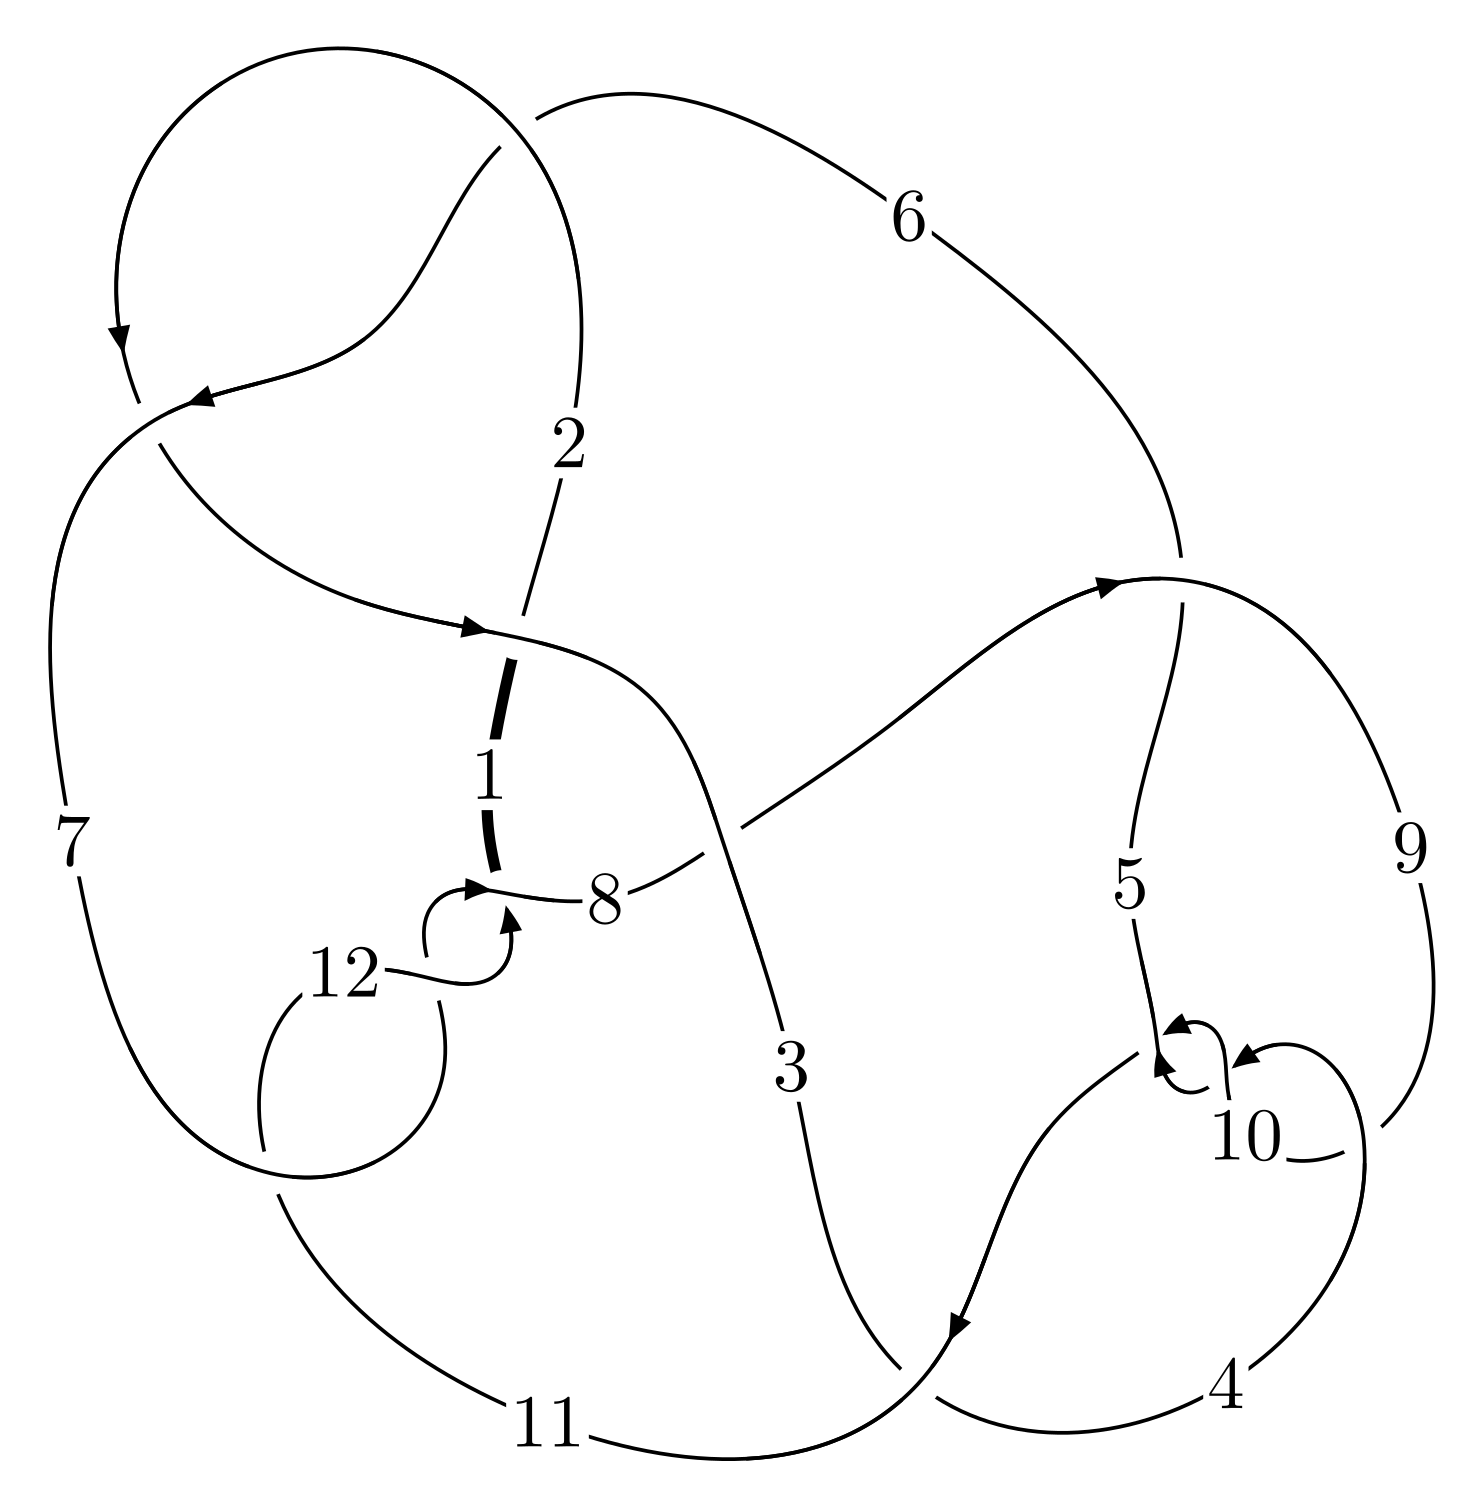
\includegraphics[width=112pt]{../../../GIT/diagram.site/Diagrams/png/2665_12n_0576.png}\\
\ \ \ A knot diagram\footnotemark}&
\allowdisplaybreaks
\textbf{Linearized knot diagam} \\
\cline{2-2}
 &
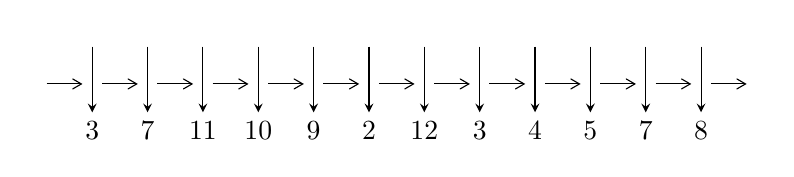
\begin{tikzpicture}[x=20pt, y=17pt]
	% nodes
	\node (C0) at (0, 0) {};
	\node (C1) at (1, 0) {};
	\node (C1U) at (1, +1) {};
	\node (C1D) at (1, -1) {3};

	\node (C2) at (2, 0) {};
	\node (C2U) at (2, +1) {};
	\node (C2D) at (2, -1) {7};

	\node (C3) at (3, 0) {};
	\node (C3U) at (3, +1) {};
	\node (C3D) at (3, -1) {11};

	\node (C4) at (4, 0) {};
	\node (C4U) at (4, +1) {};
	\node (C4D) at (4, -1) {10};

	\node (C5) at (5, 0) {};
	\node (C5U) at (5, +1) {};
	\node (C5D) at (5, -1) {9};

	\node (C6) at (6, 0) {};
	\node (C6U) at (6, +1) {};
	\node (C6D) at (6, -1) {2};

	\node (C7) at (7, 0) {};
	\node (C7U) at (7, +1) {};
	\node (C7D) at (7, -1) {12};

	\node (C8) at (8, 0) {};
	\node (C8U) at (8, +1) {};
	\node (C8D) at (8, -1) {3};

	\node (C9) at (9, 0) {};
	\node (C9U) at (9, +1) {};
	\node (C9D) at (9, -1) {4};

	\node (C10) at (10, 0) {};
	\node (C10U) at (10, +1) {};
	\node (C10D) at (10, -1) {5};

	\node (C11) at (11, 0) {};
	\node (C11U) at (11, +1) {};
	\node (C11D) at (11, -1) {7};

	\node (C12) at (12, 0) {};
	\node (C12U) at (12, +1) {};
	\node (C12D) at (12, -1) {8};
	\node (C13) at (13, 0) {};

	% arrows
	\draw[->,>={angle 60}]
	(C0) edge (C1) (C1) edge (C2) (C2) edge (C3) (C3) edge (C4) (C4) edge (C5) (C5) edge (C6) (C6) edge (C7) (C7) edge (C8) (C8) edge (C9) (C9) edge (C10) (C10) edge (C11) (C11) edge (C12) (C12) edge (C13) ;	\draw[->,>=stealth]
	(C1U) edge (C1D) (C2U) edge (C2D) (C3U) edge (C3D) (C4U) edge (C4D) (C5U) edge (C5D) (C6U) edge (C6D) (C7U) edge (C7D) (C8U) edge (C8D) (C9U) edge (C9D) (C10U) edge (C10D) (C11U) edge (C11D) (C12U) edge (C12D) ;
	\end{tikzpicture} \\
\hhline{~~} \\& 
\textbf{Solving Sequence} \\ \cline{2-2} 
 &
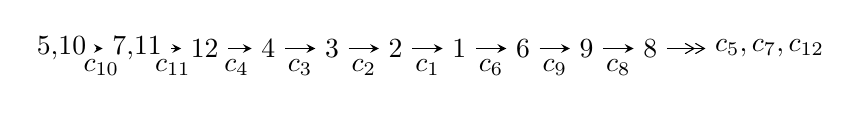
\begin{tikzpicture}[x=23pt, y=7pt]
	% node
	\node (A0) at (-1/8, 0) {5,10};
	\node (A1) at (17/16, 0) {7,11};
	\node (A2) at (17/8, 0) {12};
	\node (A3) at (25/8, 0) {4};
	\node (A4) at (33/8, 0) {3};
	\node (A5) at (41/8, 0) {2};
	\node (A6) at (49/8, 0) {1};
	\node (A7) at (57/8, 0) {6};
	\node (A8) at (65/8, 0) {9};
	\node (A9) at (73/8, 0) {8};
	\node (C1) at (1/2, -1) {$c_{10}$};
	\node (C2) at (13/8, -1) {$c_{11}$};
	\node (C3) at (21/8, -1) {$c_{4}$};
	\node (C4) at (29/8, -1) {$c_{3}$};
	\node (C5) at (37/8, -1) {$c_{2}$};
	\node (C6) at (45/8, -1) {$c_{1}$};
	\node (C7) at (53/8, -1) {$c_{6}$};
	\node (C8) at (61/8, -1) {$c_{9}$};
	\node (C9) at (69/8, -1) {$c_{8}$};
	\node (A10) at (11, 0) {$c_{5},c_{7},c_{12}$};

	% edge
	\draw[->,>=stealth]	
	(A0) edge (A1) (A1) edge (A2) (A2) edge (A3) (A3) edge (A4) (A4) edge (A5) (A5) edge (A6) (A6) edge (A7) (A7) edge (A8) (A8) edge (A9) ;
	\draw[->>,>={angle 60}]	
	(A9) edge (A10);
\end{tikzpicture} \\ 

\end{tabular} \\

\footnotetext{
The image of knot diagram is generated by the software ``\textbf{Draw programme}" developed by Andrew Bartholomew(\url{http://www.layer8.co.uk/maths/draw/index.htm\#Running-draw}), where we modified some parts for our purpose(\url{https://github.com/CATsTAILs/LinksPainter}).
}\phantom \\ \newline 
\centering \textbf{Ideals for irreducible components\footnotemark of $X_{\text{par}}$} 
 
\begin{align*}
I^u_{1}&=\langle 
-2 u^{14}+3 u^{13}+9 u^{12}-9 u^{11}-20 u^{10}+4 u^9+22 u^8+18 u^7-3 u^6-24 u^5-17 u^4+4 u^3+5 u^2+b+10 u+3,\\
\phantom{I^u_{1}}&\phantom{= \langle  }-3 u^{14}+5 u^{13}+12 u^{12}-15 u^{11}-24 u^{10}+8 u^9+24 u^8+25 u^7-34 u^5-24 u^4+5 u^3+5 u^2+2 a+17 u+4,\\
\phantom{I^u_{1}}&\phantom{= \langle  }u^{15}-3 u^{14}-2 u^{13}+11 u^{12}+2 u^{11}-16 u^{10}-6 u^9+7 u^8+14 u^7+8 u^6-10 u^5-13 u^4+u^3- u^2+6 u+2\rangle \\
I^u_{2}&=\langle 
- u^3 a- u^2 a- u^3+a u- u^2+b- a+u,\;2 u^4 a+2 u^3 a+2 u^4-3 u^2 a+2 u^3+a^2-2 a u-3 u^2+a-3 u+1,\\
\phantom{I^u_{2}}&\phantom{= \langle  }u^5+u^4-2 u^3- u^2+u-1\rangle \\
I^u_{3}&=\langle 
u^3+2 u^2+b-2 u-2,\;2 u^3+3 u^2+3 a-3 u-3,\;u^4-3 u^2+3\rangle \\
I^u_{4}&=\langle 
u^3+b,\;u^2+a+u-1,\;u^4- u^2-1\rangle \\
\\
I^v_{1}&=\langle 
a,\;b+1,\;v+1\rangle \\
\end{align*}
\raggedright * 5 irreducible components of $\dim_{\mathbb{C}}=0$, with total 34 representations.\\
\footnotetext{All coefficients of polynomials are rational numbers. But the coefficients are sometimes approximated in decimal forms when there is not enough margin.}
\newpage
\renewcommand{\arraystretch}{1}
\centering \section*{I. $I^u_{1}= \langle -2 u^{14}+3 u^{13}+\cdots+b+3,\;-3 u^{14}+5 u^{13}+\cdots+2 a+4,\;u^{15}-3 u^{14}+\cdots+6 u+2 \rangle$}
\flushleft \textbf{(i) Arc colorings}\\
\begin{tabular}{m{7pt} m{180pt} m{7pt} m{180pt} }
\flushright $a_{5}=$&$\begin{pmatrix}0\\u\end{pmatrix}$ \\
\flushright $a_{10}=$&$\begin{pmatrix}1\\0\end{pmatrix}$ \\
\flushright $a_{7}=$&$\begin{pmatrix}\frac{3}{2} u^{14}-\frac{5}{2} u^{13}+\cdots-\frac{17}{2} u-2\\2 u^{14}-3 u^{13}+\cdots-10 u-3\end{pmatrix}$ \\
\flushright $a_{11}=$&$\begin{pmatrix}1\\u^2\end{pmatrix}$ \\
\flushright $a_{12}=$&$\begin{pmatrix}\frac{1}{2} u^{14}-\frac{1}{2} u^{13}+\cdots-\frac{5}{2} u^2-\frac{7}{2} u\\2 u^{14}-3 u^{13}+\cdots-11 u-3\end{pmatrix}$ \\
\flushright $a_{4}=$&$\begin{pmatrix}u\\u\end{pmatrix}$ \\
\flushright $a_{3}=$&$\begin{pmatrix}- u^3+2 u\\- u^5+u^3+u\end{pmatrix}$ \\
\flushright $a_{2}=$&$\begin{pmatrix}\frac{1}{2} u^{14}-\frac{1}{2} u^{13}+\cdots-\frac{3}{2} u-1\\2 u^{14}-3 u^{13}+\cdots-10 u-3\end{pmatrix}$ \\
\flushright $a_{1}=$&$\begin{pmatrix}\frac{3}{2} u^{14}-\frac{3}{2} u^{13}+\cdots-\frac{19}{2} u-3\\7 u^{14}-11 u^{13}+\cdots-39 u-11\end{pmatrix}$ \\
\flushright $a_{6}=$&$\begin{pmatrix}- u^5+2 u^3- u\\- u^5+u^3+u\end{pmatrix}$ \\
\flushright $a_{9}=$&$\begin{pmatrix}- u^2+1\\- u^2\end{pmatrix}$ \\
\flushright $a_{8}=$&$\begin{pmatrix}u^{10}-5 u^8+8 u^6-3 u^4-3 u^2+1\\u^{12}-4 u^{10}+4 u^8+2 u^6-3 u^4-2 u^2\end{pmatrix}$\\&\end{tabular}
\flushleft \textbf{(ii) Obstruction class $= -1$}\\~\\
\flushleft \textbf{(iii) Cusp Shapes $= -2 u^{12}+10 u^{10}+6 u^9-18 u^8-24 u^7+2 u^6+30 u^5+30 u^4+2 u^3-22 u^2-20 u-24$}\\~\\
\newpage\renewcommand{\arraystretch}{1}
\flushleft \textbf{(iv) u-Polynomials at the component}\newline \\
\begin{tabular}{m{50pt}|m{274pt}}
Crossings & \hspace{64pt}u-Polynomials at each crossing \\
\hline $$\begin{aligned}c_{1}\end{aligned}$$&$\begin{aligned}
&u^{15}+27 u^{14}+\cdots+21 u+1
\end{aligned}$\\
\hline $$\begin{aligned}c_{2},c_{6},c_{7}\\c_{11},c_{12}\end{aligned}$$&$\begin{aligned}
&u^{15}- u^{14}+\cdots-3 u-1
\end{aligned}$\\
\hline $$\begin{aligned}c_{3},c_{5}\end{aligned}$$&$\begin{aligned}
&u^{15}+9 u^{14}+\cdots+166 u+22
\end{aligned}$\\
\hline $$\begin{aligned}c_{4},c_{9},c_{10}\end{aligned}$$&$\begin{aligned}
&u^{15}-3 u^{14}+\cdots+6 u+2
\end{aligned}$\\
\hline $$\begin{aligned}c_{8}\end{aligned}$$&$\begin{aligned}
&u^{15}+3 u^{14}+\cdots+326 u+178
\end{aligned}$\\
\hline
\end{tabular}\\~\\
\newpage\renewcommand{\arraystretch}{1}
\flushleft \textbf{(v) Riley Polynomials at the component}\newline \\
\begin{tabular}{m{50pt}|m{274pt}}
Crossings & \hspace{64pt}Riley Polynomials at each crossing \\
\hline $$\begin{aligned}c_{1}\end{aligned}$$&$\begin{aligned}
&y^{15}-91 y^{14}+\cdots+125 y-1
\end{aligned}$\\
\hline $$\begin{aligned}c_{2},c_{6},c_{7}\\c_{11},c_{12}\end{aligned}$$&$\begin{aligned}
&y^{15}-27 y^{14}+\cdots+21 y-1
\end{aligned}$\\
\hline $$\begin{aligned}c_{3},c_{5}\end{aligned}$$&$\begin{aligned}
&y^{15}+7 y^{14}+\cdots+5336 y-484
\end{aligned}$\\
\hline $$\begin{aligned}c_{4},c_{9},c_{10}\end{aligned}$$&$\begin{aligned}
&y^{15}-13 y^{14}+\cdots+40 y-4
\end{aligned}$\\
\hline $$\begin{aligned}c_{8}\end{aligned}$$&$\begin{aligned}
&y^{15}-73 y^{14}+\cdots-18680 y-31684
\end{aligned}$\\
\hline
\end{tabular}\\~\\
\newpage\flushleft \textbf{(vi) Complex Volumes and Cusp Shapes}
$$\begin{array}{c|c|c}  
\text{Solutions to }I^u_{1}& \I (\text{vol} + \sqrt{-1}CS) & \text{Cusp shape}\\
 \hline 
\begin{aligned}
u &= -0.933456 + 0.545096 I \\
a &= \phantom{-}1.35570 - 0.53655 I \\
b &= \phantom{-}2.15361 - 1.54045 I\end{aligned}
 & -16.1665 - 1.0397 I & -16.7131 - 1.0217 I \\ \hline\begin{aligned}
u &= -0.933456 - 0.545096 I \\
a &= \phantom{-}1.35570 + 0.53655 I \\
b &= \phantom{-}2.15361 + 1.54045 I\end{aligned}
 & -16.1665 + 1.0397 I & -16.7131 + 1.0217 I \\ \hline\begin{aligned}
u &= -0.269872 + 0.870864 I \\
a &= -2.11208 + 1.63104 I \\
b &= \phantom{-}0.313757 + 0.153473 I\end{aligned}
 & -14.1086 + 6.0067 I & -14.4990 - 3.2830 I \\ \hline\begin{aligned}
u &= -0.269872 - 0.870864 I \\
a &= -2.11208 - 1.63104 I \\
b &= \phantom{-}0.313757 - 0.153473 I\end{aligned}
 & -14.1086 - 6.0067 I & -14.4990 + 3.2830 I \\ \hline\begin{aligned}
u &= -0.027957 + 0.721725 I \\
a &= \phantom{-}0.449087 - 1.012280 I \\
b &= \phantom{-}0.210760 + 0.156059 I\end{aligned}
 & \phantom{-}2.42887 + 1.37514 I & -7.68727 - 5.21222 I \\ \hline\begin{aligned}
u &= -0.027957 - 0.721725 I \\
a &= \phantom{-}0.449087 + 1.012280 I \\
b &= \phantom{-}0.210760 - 0.156059 I\end{aligned}
 & \phantom{-}2.42887 - 1.37514 I & -7.68727 + 5.21222 I \\ \hline\begin{aligned}
u &= -1.269950 + 0.268466 I \\
a &= -0.329692 - 0.304561 I \\
b &= -1.118860 - 0.755791 I\end{aligned}
 & -1.39715 + 2.17673 I & -12.08651 + 0.76556 I \\ \hline\begin{aligned}
u &= -1.269950 - 0.268466 I \\
a &= -0.329692 + 0.304561 I \\
b &= -1.118860 + 0.755791 I\end{aligned}
 & -1.39715 - 2.17673 I & -12.08651 - 0.76556 I \\ \hline\begin{aligned}
u &= \phantom{-}1.31650\phantom{ +0.000000I} \\
a &= -0.714575\phantom{ +0.000000I} \\
b &= -0.728053\phantom{ +0.000000I}\end{aligned}
 & -5.38119\phantom{ +0.000000I} & -18.1900\phantom{ +0.000000I} \\ \hline\begin{aligned}
u &= \phantom{-}1.289830 + 0.310526 I \\
a &= \phantom{-}0.355754 - 0.895009 I \\
b &= \phantom{-}0.71766 - 1.39362 I\end{aligned}
 & -1.68505 - 5.12171 I & -12.9962 + 7.9827 I\\
 \hline 
 \end{array}$$\newpage$$\begin{array}{c|c|c}  
\text{Solutions to }I^u_{1}& \I (\text{vol} + \sqrt{-1}CS) & \text{Cusp shape}\\
 \hline 
\begin{aligned}
u &= \phantom{-}1.289830 - 0.310526 I \\
a &= \phantom{-}0.355754 + 0.895009 I \\
b &= \phantom{-}0.71766 + 1.39362 I\end{aligned}
 & -1.68505 + 5.12171 I & -12.9962 - 7.9827 I \\ \hline\begin{aligned}
u &= \phantom{-}1.43481 + 0.35867 I \\
a &= \phantom{-}0.18363 + 1.96597 I \\
b &= \phantom{-}0.25436 + 4.36591 I\end{aligned}
 & -19.5375 - 10.4475 I & -18.0265 + 4.5376 I \\ \hline\begin{aligned}
u &= \phantom{-}1.43481 - 0.35867 I \\
a &= \phantom{-}0.18363 - 1.96597 I \\
b &= \phantom{-}0.25436 - 4.36591 I\end{aligned}
 & -19.5375 + 10.4475 I & -18.0265 - 4.5376 I \\ \hline\begin{aligned}
u &= \phantom{-}1.53735\phantom{ +0.000000I} \\
a &= \phantom{-}0.453716\phantom{ +0.000000I} \\
b &= -1.08285\phantom{ +0.000000I}\end{aligned}
 & \phantom{-}14.6944\phantom{ +0.000000I} & -19.9400\phantom{ +0.000000I} \\ \hline\begin{aligned}
u &= -0.300672\phantom{ +0.000000I} \\
a &= \phantom{-}0.456072\phantom{ +0.000000I} \\
b &= -0.251678\phantom{ +0.000000I}\end{aligned}
 & -0.497687\phantom{ +0.000000I} & -19.8530\phantom{ +0.000000I}\\
 \hline 
 \end{array}$$\newpage\newpage\renewcommand{\arraystretch}{1}
\centering \section*{II. $I^u_{2}= \langle - u^3 a- u^2 a- u^3+a u- u^2+b- a+u,\;2 u^4 a+2 u^4+\cdots+a+1,\;u^5+u^4-2 u^3- u^2+u-1 \rangle$}
\flushleft \textbf{(i) Arc colorings}\\
\begin{tabular}{m{7pt} m{180pt} m{7pt} m{180pt} }
\flushright $a_{5}=$&$\begin{pmatrix}0\\u\end{pmatrix}$ \\
\flushright $a_{10}=$&$\begin{pmatrix}1\\0\end{pmatrix}$ \\
\flushright $a_{7}=$&$\begin{pmatrix}a\\u^3 a+u^2 a+u^3- a u+u^2+a- u\end{pmatrix}$ \\
\flushright $a_{11}=$&$\begin{pmatrix}1\\u^2\end{pmatrix}$ \\
\flushright $a_{12}=$&$\begin{pmatrix}- u^4 a- u^3 a+u^2 a-2 u^3+a u- u^2+3 u+1\\- u^4 a+u^4+u^2 a- u^3- u^2+2 u\end{pmatrix}$ \\
\flushright $a_{4}=$&$\begin{pmatrix}u\\u\end{pmatrix}$ \\
\flushright $a_{3}=$&$\begin{pmatrix}- u^3+2 u\\u^4- u^3- u^2+2 u-1\end{pmatrix}$ \\
\flushright $a_{2}=$&$\begin{pmatrix}u^3 a+u^2 a+u^3- a u+u^2- u\\u^3 a+u^2 a+u^3- a u+u^2+a- u\end{pmatrix}$ \\
\flushright $a_{1}=$&$\begin{pmatrix}- u^4 a+u^3 a+3 u^2 a+2 u^3- a u+u^2-3 u+1\\-2 u^4 a+2 u^3 a-2 u^4+4 u^2 a+2 u^3-3 a u+4 u^2+2 a-4 u+2\end{pmatrix}$ \\
\flushright $a_{6}=$&$\begin{pmatrix}u^4- u^2-1\\u^4- u^3- u^2+2 u-1\end{pmatrix}$ \\
\flushright $a_{9}=$&$\begin{pmatrix}- u^2+1\\- u^2\end{pmatrix}$ \\
\flushright $a_{8}=$&$\begin{pmatrix}-2 u^2+2\\-2 u^2+u\end{pmatrix}$\\&\end{tabular}
\flushleft \textbf{(ii) Obstruction class $= -1$}\\~\\
\flushleft \textbf{(iii) Cusp Shapes $= -4 u^3+8 u-18$}\\~\\
\newpage\renewcommand{\arraystretch}{1}
\flushleft \textbf{(iv) u-Polynomials at the component}\newline \\
\begin{tabular}{m{50pt}|m{274pt}}
Crossings & \hspace{64pt}u-Polynomials at each crossing \\
\hline $$\begin{aligned}c_{1}\end{aligned}$$&$\begin{aligned}
&u^{10}+13 u^9+\cdots+536 u+49
\end{aligned}$\\
\hline $$\begin{aligned}c_{2},c_{6},c_{7}\\c_{11},c_{12}\end{aligned}$$&$\begin{aligned}
&u^{10}- u^9-6 u^8+4 u^7+18 u^6-8 u^5-31 u^4+13 u^3+28 u^2-12 u-7
\end{aligned}$\\
\hline $$\begin{aligned}c_{3},c_{5}\end{aligned}$$&$\begin{aligned}
&(u^5-3 u^4+4 u^3- u^2- u+1)^2
\end{aligned}$\\
\hline $$\begin{aligned}c_{4},c_{9},c_{10}\end{aligned}$$&$\begin{aligned}
&(u^5+u^4-2 u^3- u^2+u-1)^2
\end{aligned}$\\
\hline $$\begin{aligned}c_{8}\end{aligned}$$&$\begin{aligned}
&(u^5- u^4+2 u^3- u^2+u-1)^2
\end{aligned}$\\
\hline
\end{tabular}\\~\\
\newpage\renewcommand{\arraystretch}{1}
\flushleft \textbf{(v) Riley Polynomials at the component}\newline \\
\begin{tabular}{m{50pt}|m{274pt}}
Crossings & \hspace{64pt}Riley Polynomials at each crossing \\
\hline $$\begin{aligned}c_{1}\end{aligned}$$&$\begin{aligned}
&y^{10}-9 y^9+\cdots-137356 y+2401
\end{aligned}$\\
\hline $$\begin{aligned}c_{2},c_{6},c_{7}\\c_{11},c_{12}\end{aligned}$$&$\begin{aligned}
&y^{10}-13 y^9+\cdots-536 y+49
\end{aligned}$\\
\hline $$\begin{aligned}c_{3},c_{5}\end{aligned}$$&$\begin{aligned}
&(y^5- y^4+8 y^3-3 y^2+3 y-1)^2
\end{aligned}$\\
\hline $$\begin{aligned}c_{4},c_{9},c_{10}\end{aligned}$$&$\begin{aligned}
&(y^5-5 y^4+8 y^3-3 y^2- y-1)^2
\end{aligned}$\\
\hline $$\begin{aligned}c_{8}\end{aligned}$$&$\begin{aligned}
&(y^5+3 y^4+4 y^3+y^2- y-1)^2
\end{aligned}$\\
\hline
\end{tabular}\\~\\
\newpage\flushleft \textbf{(vi) Complex Volumes and Cusp Shapes}
$$\begin{array}{c|c|c}  
\text{Solutions to }I^u_{2}& \I (\text{vol} + \sqrt{-1}CS) & \text{Cusp shape}\\
 \hline 
\begin{aligned}
u &= \phantom{-}1.21774\phantom{ +0.000000I} \\
a &= -0.591829\phantom{ +0.000000I} \\
b &= \phantom{-}0.253452\phantom{ +0.000000I}\end{aligned}
 & -5.69095\phantom{ +0.000000I} & -15.4810\phantom{ +0.000000I} \\ \hline\begin{aligned}
u &= \phantom{-}1.21774\phantom{ +0.000000I} \\
a &= -1.53344\phantom{ +0.000000I} \\
b &= -2.63815\phantom{ +0.000000I}\end{aligned}
 & -5.69095\phantom{ +0.000000I} & -15.4810\phantom{ +0.000000I} \\ \hline\begin{aligned}
u &= \phantom{-}0.309916 + 0.549911 I \\
a &= -1.031800 - 0.275887 I \\
b &= -1.067230 - 0.057202 I\end{aligned}
 & -3.61897 - 1.53058 I & -14.5151 + 4.4306 I \\ \hline\begin{aligned}
u &= \phantom{-}0.309916 + 0.549911 I \\
a &= \phantom{-}0.68255 + 2.69529 I \\
b &= -0.024468 + 0.261280 I\end{aligned}
 & -3.61897 - 1.53058 I & -14.5151 + 4.4306 I \\ \hline\begin{aligned}
u &= \phantom{-}0.309916 - 0.549911 I \\
a &= -1.031800 + 0.275887 I \\
b &= -1.067230 + 0.057202 I\end{aligned}
 & -3.61897 + 1.53058 I & -14.5151 - 4.4306 I \\ \hline\begin{aligned}
u &= \phantom{-}0.309916 - 0.549911 I \\
a &= \phantom{-}0.68255 - 2.69529 I \\
b &= -0.024468 - 0.261280 I\end{aligned}
 & -3.61897 + 1.53058 I & -14.5151 - 4.4306 I \\ \hline\begin{aligned}
u &= -1.41878 + 0.21917 I \\
a &= -0.310913 - 0.768355 I \\
b &= \phantom{-}0.556241 - 1.005760 I\end{aligned}
 & -9.16243 + 4.40083 I & -18.7443 - 3.4986 I \\ \hline\begin{aligned}
u &= -1.41878 + 0.21917 I \\
a &= \phantom{-}0.72280 + 1.60293 I \\
b &= \phantom{-}1.22781 + 3.58963 I\end{aligned}
 & -9.16243 + 4.40083 I & -18.7443 - 3.4986 I \\ \hline\begin{aligned}
u &= -1.41878 - 0.21917 I \\
a &= -0.310913 + 0.768355 I \\
b &= \phantom{-}0.556241 + 1.005760 I\end{aligned}
 & -9.16243 - 4.40083 I & -18.7443 + 3.4986 I \\ \hline\begin{aligned}
u &= -1.41878 - 0.21917 I \\
a &= \phantom{-}0.72280 - 1.60293 I \\
b &= \phantom{-}1.22781 - 3.58963 I\end{aligned}
 & -9.16243 - 4.40083 I & -18.7443 + 3.4986 I\\
 \hline 
 \end{array}$$\newpage\newpage\renewcommand{\arraystretch}{1}
\centering \section*{III. $I^u_{3}= \langle u^3+2 u^2+b-2 u-2,\;2 u^3+3 u^2+3 a-3 u-3,\;u^4-3 u^2+3 \rangle$}
\flushleft \textbf{(i) Arc colorings}\\
\begin{tabular}{m{7pt} m{180pt} m{7pt} m{180pt} }
\flushright $a_{5}=$&$\begin{pmatrix}0\\u\end{pmatrix}$ \\
\flushright $a_{10}=$&$\begin{pmatrix}1\\0\end{pmatrix}$ \\
\flushright $a_{7}=$&$\begin{pmatrix}-\frac{2}{3} u^3- u^2+u+1\\- u^3-2 u^2+2 u+2\end{pmatrix}$ \\
\flushright $a_{11}=$&$\begin{pmatrix}1\\u^2\end{pmatrix}$ \\
\flushright $a_{12}=$&$\begin{pmatrix}\frac{2}{3} u^3+u^2- u\\u^3+3 u^2-2 u-2\end{pmatrix}$ \\
\flushright $a_{4}=$&$\begin{pmatrix}u\\u\end{pmatrix}$ \\
\flushright $a_{3}=$&$\begin{pmatrix}- u^3+2 u\\-2 u^3+4 u\end{pmatrix}$ \\
\flushright $a_{2}=$&$\begin{pmatrix}-\frac{1}{3} u^3+u^2+u-1\\- u^3+2 u^2+2 u-2\end{pmatrix}$ \\
\flushright $a_{1}=$&$\begin{pmatrix}\frac{2}{3} u^3+u^2- u-1\\u^3+2 u^2-2 u-2\end{pmatrix}$ \\
\flushright $a_{6}=$&$\begin{pmatrix}- u^3+2 u\\-2 u^3+4 u\end{pmatrix}$ \\
\flushright $a_{9}=$&$\begin{pmatrix}- u^2+1\\- u^2\end{pmatrix}$ \\
\flushright $a_{8}=$&$\begin{pmatrix}1\\u^2\end{pmatrix}$\\&\end{tabular}
\flushleft \textbf{(ii) Obstruction class $= 1$}\\~\\
\flushleft \textbf{(iii) Cusp Shapes $= 4 u^2-24$}\\~\\
\newpage\renewcommand{\arraystretch}{1}
\flushleft \textbf{(iv) u-Polynomials at the component}\newline \\
\begin{tabular}{m{50pt}|m{274pt}}
Crossings & \hspace{64pt}u-Polynomials at each crossing \\
\hline $$\begin{aligned}c_{1},c_{2},c_{7}\end{aligned}$$&$\begin{aligned}
&(u-1)^4
\end{aligned}$\\
\hline $$\begin{aligned}c_{3},c_{5},c_{8}\end{aligned}$$&$\begin{aligned}
&u^4+3 u^2+3
\end{aligned}$\\
\hline $$\begin{aligned}c_{4},c_{9},c_{10}\end{aligned}$$&$\begin{aligned}
&u^4-3 u^2+3
\end{aligned}$\\
\hline $$\begin{aligned}c_{6},c_{11},c_{12}\end{aligned}$$&$\begin{aligned}
&(u+1)^4
\end{aligned}$\\
\hline
\end{tabular}\\~\\
\newpage\renewcommand{\arraystretch}{1}
\flushleft \textbf{(v) Riley Polynomials at the component}\newline \\
\begin{tabular}{m{50pt}|m{274pt}}
Crossings & \hspace{64pt}Riley Polynomials at each crossing \\
\hline $$\begin{aligned}c_{1},c_{2},c_{6}\\c_{7},c_{11},c_{12}\end{aligned}$$&$\begin{aligned}
&(y-1)^4
\end{aligned}$\\
\hline $$\begin{aligned}c_{3},c_{5},c_{8}\end{aligned}$$&$\begin{aligned}
&(y^2+3 y+3)^2
\end{aligned}$\\
\hline $$\begin{aligned}c_{4},c_{9},c_{10}\end{aligned}$$&$\begin{aligned}
&(y^2-3 y+3)^2
\end{aligned}$\\
\hline
\end{tabular}\\~\\
\newpage\flushleft \textbf{(vi) Complex Volumes and Cusp Shapes}
$$\begin{array}{c|c|c}  
\text{Solutions to }I^u_{3}& \I (\text{vol} + \sqrt{-1}CS) & \text{Cusp shape}\\
 \hline 
\begin{aligned}
u &= \phantom{-}1.271230 + 0.340625 I \\
a &= -0.30334 - 1.59997 I \\
b &= -0.06940 - 2.66266 I\end{aligned}
 & -3.28987 - 4.05977 I & -18.0000 + 3.4641 I \\ \hline\begin{aligned}
u &= \phantom{-}1.271230 - 0.340625 I \\
a &= -0.30334 + 1.59997 I \\
b &= -0.06940 + 2.66266 I\end{aligned}
 & -3.28987 + 4.05977 I & -18.0000 - 3.4641 I \\ \hline\begin{aligned}
u &= -1.271230 + 0.340625 I \\
a &= -0.696660 + 0.132080 I \\
b &= -1.93060 + 0.80145 I\end{aligned}
 & -3.28987 + 4.05977 I & -18.0000 - 3.4641 I \\ \hline\begin{aligned}
u &= -1.271230 - 0.340625 I \\
a &= -0.696660 - 0.132080 I \\
b &= -1.93060 - 0.80145 I\end{aligned}
 & -3.28987 - 4.05977 I & -18.0000 + 3.4641 I\\
 \hline 
 \end{array}$$\newpage\newpage\renewcommand{\arraystretch}{1}
\centering \section*{IV. $I^u_{4}= \langle u^3+b,\;u^2+a+u-1,\;u^4- u^2-1 \rangle$}
\flushleft \textbf{(i) Arc colorings}\\
\begin{tabular}{m{7pt} m{180pt} m{7pt} m{180pt} }
\flushright $a_{5}=$&$\begin{pmatrix}0\\u\end{pmatrix}$ \\
\flushright $a_{10}=$&$\begin{pmatrix}1\\0\end{pmatrix}$ \\
\flushright $a_{7}=$&$\begin{pmatrix}- u^2- u+1\\- u^3\end{pmatrix}$ \\
\flushright $a_{11}=$&$\begin{pmatrix}1\\u^2\end{pmatrix}$ \\
\flushright $a_{12}=$&$\begin{pmatrix}- u^2- u+2\\- u^3+u^2\end{pmatrix}$ \\
\flushright $a_{4}=$&$\begin{pmatrix}u\\u\end{pmatrix}$ \\
\flushright $a_{3}=$&$\begin{pmatrix}- u^3+2 u\\0\end{pmatrix}$ \\
\flushright $a_{2}=$&$\begin{pmatrix}- u^3- u^2+u+1\\- u^3\end{pmatrix}$ \\
\flushright $a_{1}=$&$\begin{pmatrix}- u^2- u+1\\- u^3\end{pmatrix}$ \\
\flushright $a_{6}=$&$\begin{pmatrix}u^3-2 u\\0\end{pmatrix}$ \\
\flushright $a_{9}=$&$\begin{pmatrix}- u^2+1\\- u^2\end{pmatrix}$ \\
\flushright $a_{8}=$&$\begin{pmatrix}-1\\- u^2\end{pmatrix}$\\&\end{tabular}
\flushleft \textbf{(ii) Obstruction class $= 1$}\\~\\
\flushleft \textbf{(iii) Cusp Shapes $= -4 u^2-16$}\\~\\
\newpage\renewcommand{\arraystretch}{1}
\flushleft \textbf{(iv) u-Polynomials at the component}\newline \\
\begin{tabular}{m{50pt}|m{274pt}}
Crossings & \hspace{64pt}u-Polynomials at each crossing \\
\hline $$\begin{aligned}c_{1},c_{6},c_{11}\\c_{12}\end{aligned}$$&$\begin{aligned}
&(u-1)^4
\end{aligned}$\\
\hline $$\begin{aligned}c_{2},c_{7}\end{aligned}$$&$\begin{aligned}
&(u+1)^4
\end{aligned}$\\
\hline $$\begin{aligned}c_{3},c_{5},c_{8}\end{aligned}$$&$\begin{aligned}
&u^4+u^2-1
\end{aligned}$\\
\hline $$\begin{aligned}c_{4},c_{9},c_{10}\end{aligned}$$&$\begin{aligned}
&u^4- u^2-1
\end{aligned}$\\
\hline
\end{tabular}\\~\\
\newpage\renewcommand{\arraystretch}{1}
\flushleft \textbf{(v) Riley Polynomials at the component}\newline \\
\begin{tabular}{m{50pt}|m{274pt}}
Crossings & \hspace{64pt}Riley Polynomials at each crossing \\
\hline $$\begin{aligned}c_{1},c_{2},c_{6}\\c_{7},c_{11},c_{12}\end{aligned}$$&$\begin{aligned}
&(y-1)^4
\end{aligned}$\\
\hline $$\begin{aligned}c_{3},c_{5},c_{8}\end{aligned}$$&$\begin{aligned}
&(y^2+y-1)^2
\end{aligned}$\\
\hline $$\begin{aligned}c_{4},c_{9},c_{10}\end{aligned}$$&$\begin{aligned}
&(y^2- y-1)^2
\end{aligned}$\\
\hline
\end{tabular}\\~\\
\newpage\flushleft \textbf{(vi) Complex Volumes and Cusp Shapes}
$$\begin{array}{c|c|c}  
\text{Solutions to }I^u_{4}& \I (\text{vol} + \sqrt{-1}CS) & \text{Cusp shape}\\
 \hline 
\begin{aligned}
u &= \phantom{-0.000000 -}0.786151 I \\
a &= \phantom{-}1.61803 - 0.78615 I \\
b &= \phantom{-0.000000 -}0.485868 I\end{aligned}
 & \phantom{-}0.657974\phantom{ +0.000000I} & -13.5280\phantom{ +0.000000I} \\ \hline\begin{aligned}
u &= \phantom{-0.000000 } -0.786151 I \\
a &= \phantom{-}1.61803 + 0.78615 I \\
b &= \phantom{-0.000000 } -0.485868 I\end{aligned}
 & \phantom{-}0.657974\phantom{ +0.000000I} & -13.5280\phantom{ +0.000000I} \\ \hline\begin{aligned}
u &= \phantom{-}1.27202\phantom{ +0.000000I} \\
a &= -1.89005\phantom{ +0.000000I} \\
b &= -2.05817\phantom{ +0.000000I}\end{aligned}
 & -7.23771\phantom{ +0.000000I} & -22.4720\phantom{ +0.000000I} \\ \hline\begin{aligned}
u &= -1.27202\phantom{ +0.000000I} \\
a &= \phantom{-}0.653986\phantom{ +0.000000I} \\
b &= \phantom{-}2.05817\phantom{ +0.000000I}\end{aligned}
 & -7.23771\phantom{ +0.000000I} & -22.4720\phantom{ +0.000000I}\\
 \hline 
 \end{array}$$\newpage\newpage\renewcommand{\arraystretch}{1}
\centering \section*{V. $I^v_{1}= \langle a,\;b+1,\;v+1 \rangle$}
\flushleft \textbf{(i) Arc colorings}\\
\begin{tabular}{m{7pt} m{180pt} m{7pt} m{180pt} }
\flushright $a_{5}=$&$\begin{pmatrix}-1\\0\end{pmatrix}$ \\
\flushright $a_{10}=$&$\begin{pmatrix}1\\0\end{pmatrix}$ \\
\flushright $a_{7}=$&$\begin{pmatrix}0\\-1\end{pmatrix}$ \\
\flushright $a_{11}=$&$\begin{pmatrix}1\\0\end{pmatrix}$ \\
\flushright $a_{12}=$&$\begin{pmatrix}1\\1\end{pmatrix}$ \\
\flushright $a_{4}=$&$\begin{pmatrix}-1\\0\end{pmatrix}$ \\
\flushright $a_{3}=$&$\begin{pmatrix}-1\\0\end{pmatrix}$ \\
\flushright $a_{2}=$&$\begin{pmatrix}-1\\1\end{pmatrix}$ \\
\flushright $a_{1}=$&$\begin{pmatrix}0\\1\end{pmatrix}$ \\
\flushright $a_{6}=$&$\begin{pmatrix}-1\\0\end{pmatrix}$ \\
\flushright $a_{9}=$&$\begin{pmatrix}1\\0\end{pmatrix}$ \\
\flushright $a_{8}=$&$\begin{pmatrix}1\\0\end{pmatrix}$\\&\end{tabular}
\flushleft \textbf{(ii) Obstruction class $= 1$}\\~\\
\flushleft \textbf{(iii) Cusp Shapes $= -12$}\\~\\
\newpage\renewcommand{\arraystretch}{1}
\flushleft \textbf{(iv) u-Polynomials at the component}\newline \\
\begin{tabular}{m{50pt}|m{274pt}}
Crossings & \hspace{64pt}u-Polynomials at each crossing \\
\hline $$\begin{aligned}c_{1},c_{2},c_{7}\end{aligned}$$&$\begin{aligned}
&u-1
\end{aligned}$\\
\hline $$\begin{aligned}c_{3},c_{4},c_{5}\\c_{8},c_{9},c_{10}\end{aligned}$$&$\begin{aligned}
&u
\end{aligned}$\\
\hline $$\begin{aligned}c_{6},c_{11},c_{12}\end{aligned}$$&$\begin{aligned}
&u+1
\end{aligned}$\\
\hline
\end{tabular}\\~\\
\newpage\renewcommand{\arraystretch}{1}
\flushleft \textbf{(v) Riley Polynomials at the component}\newline \\
\begin{tabular}{m{50pt}|m{274pt}}
Crossings & \hspace{64pt}Riley Polynomials at each crossing \\
\hline $$\begin{aligned}c_{1},c_{2},c_{6}\\c_{7},c_{11},c_{12}\end{aligned}$$&$\begin{aligned}
&y-1
\end{aligned}$\\
\hline $$\begin{aligned}c_{3},c_{4},c_{5}\\c_{8},c_{9},c_{10}\end{aligned}$$&$\begin{aligned}
&y
\end{aligned}$\\
\hline
\end{tabular}\\~\\
\newpage\flushleft \textbf{(vi) Complex Volumes and Cusp Shapes}
$$\begin{array}{c|c|c}  
\text{Solutions to }I^v_{1}& \I (\text{vol} + \sqrt{-1}CS) & \text{Cusp shape}\\
 \hline 
\begin{aligned}
v &= -1.00000\phantom{ +0.000000I} \\
a &= \phantom{-0.000000 } 0 \\
b &= -1.00000\phantom{ +0.000000I}\end{aligned}
 & -3.28987\phantom{ +0.000000I} & -12.0000\phantom{ +0.000000I}\\
 \hline 
 \end{array}$$\newpage
\newpage\renewcommand{\arraystretch}{1}
\centering \section*{ VI. u-Polynomials}
\begin{tabular}{m{50pt}|m{274pt}}
Crossings & \hspace{64pt}u-Polynomials at each crossing \\
\hline $$\begin{aligned}c_{1}\end{aligned}$$&$\begin{aligned}
&((u-1)^9)(u^{10}+13 u^{9}+\cdots+536 u+49)(u^{15}+27 u^{14}+\cdots+21 u+1)
\end{aligned}$\\
\hline $$\begin{aligned}c_{2},c_{7}\end{aligned}$$&$\begin{aligned}
&(u-1)^5(u+1)^4\\
&\cdot(u^{10}- u^9-6 u^8+4 u^7+18 u^6-8 u^5-31 u^4+13 u^3+28 u^2-12 u-7)\\
&\cdot(u^{15}- u^{14}+\cdots-3 u-1)
\end{aligned}$\\
\hline $$\begin{aligned}c_{3},c_{5}\end{aligned}$$&$\begin{aligned}
&u(u^4+u^2-1)(u^4+3 u^2+3)(u^5-3 u^4+4 u^3- u^2- u+1)^2\\
&\cdot(u^{15}+9 u^{14}+\cdots+166 u+22)
\end{aligned}$\\
\hline $$\begin{aligned}c_{4},c_{9},c_{10}\end{aligned}$$&$\begin{aligned}
&u(u^4-3 u^2+3)(u^4- u^2-1)(u^5+u^4-2 u^3- u^2+u-1)^2\\
&\cdot(u^{15}-3 u^{14}+\cdots+6 u+2)
\end{aligned}$\\
\hline $$\begin{aligned}c_{6},c_{11},c_{12}\end{aligned}$$&$\begin{aligned}
&(u-1)^4(u+1)^5\\
&\cdot(u^{10}- u^9-6 u^8+4 u^7+18 u^6-8 u^5-31 u^4+13 u^3+28 u^2-12 u-7)\\
&\cdot(u^{15}- u^{14}+\cdots-3 u-1)
\end{aligned}$\\
\hline $$\begin{aligned}c_{8}\end{aligned}$$&$\begin{aligned}
&u(u^4+u^2-1)(u^4+3 u^2+3)(u^5- u^4+2 u^3- u^2+u-1)^2\\
&\cdot(u^{15}+3 u^{14}+\cdots+326 u+178)
\end{aligned}$\\
\hline
\end{tabular}\newpage\renewcommand{\arraystretch}{1}
\centering \section*{ VII. Riley Polynomials}
\begin{tabular}{m{50pt}|m{274pt}}
Crossings & \hspace{64pt}Riley Polynomials at each crossing \\
\hline $$\begin{aligned}c_{1}\end{aligned}$$&$\begin{aligned}
&((y-1)^9)(y^{10}-9 y^9+\cdots-137356 y+2401)\\
&\cdot(y^{15}-91 y^{14}+\cdots+125 y-1)
\end{aligned}$\\
\hline $$\begin{aligned}c_{2},c_{6},c_{7}\\c_{11},c_{12}\end{aligned}$$&$\begin{aligned}
&((y-1)^9)(y^{10}-13 y^{9}+\cdots-536 y+49)(y^{15}-27 y^{14}+\cdots+21 y-1)
\end{aligned}$\\
\hline $$\begin{aligned}c_{3},c_{5}\end{aligned}$$&$\begin{aligned}
&y(y^2+y-1)^2(y^2+3 y+3)^2(y^5- y^4+8 y^3-3 y^2+3 y-1)^2\\
&\cdot(y^{15}+7 y^{14}+\cdots+5336 y-484)
\end{aligned}$\\
\hline $$\begin{aligned}c_{4},c_{9},c_{10}\end{aligned}$$&$\begin{aligned}
&y(y^2-3 y+3)^2(y^2- y-1)^2(y^5-5 y^4+8 y^3-3 y^2- y-1)^2\\
&\cdot(y^{15}-13 y^{14}+\cdots+40 y-4)
\end{aligned}$\\
\hline $$\begin{aligned}c_{8}\end{aligned}$$&$\begin{aligned}
&y(y^2+y-1)^2(y^2+3 y+3)^2(y^5+3 y^4+4 y^3+y^2- y-1)^2\\
&\cdot(y^{15}-73 y^{14}+\cdots-18680 y-31684)
\end{aligned}$\\
\hline
\end{tabular}
\vskip 2pc
\end{document}